\documentclass{article}

\usepackage{graphicx}
\usepackage{tikz}
\usepackage{tikzsymbols}
\usetikzlibrary{calc,patterns,shapes.geometric}
\pagestyle{empty}
\usepackage[margin=0pt]{geometry}
\geometry{papersize={14in,12in}}

\def\centerarc[#1](#2)(#3:#4:#5){\draw[#1] ($(#2)+({#5*cos(#3)},{#5*sin(#3)})$) arc (#3:#4:#5);}

\begin{document}
	\begin{figure}
		\centering
		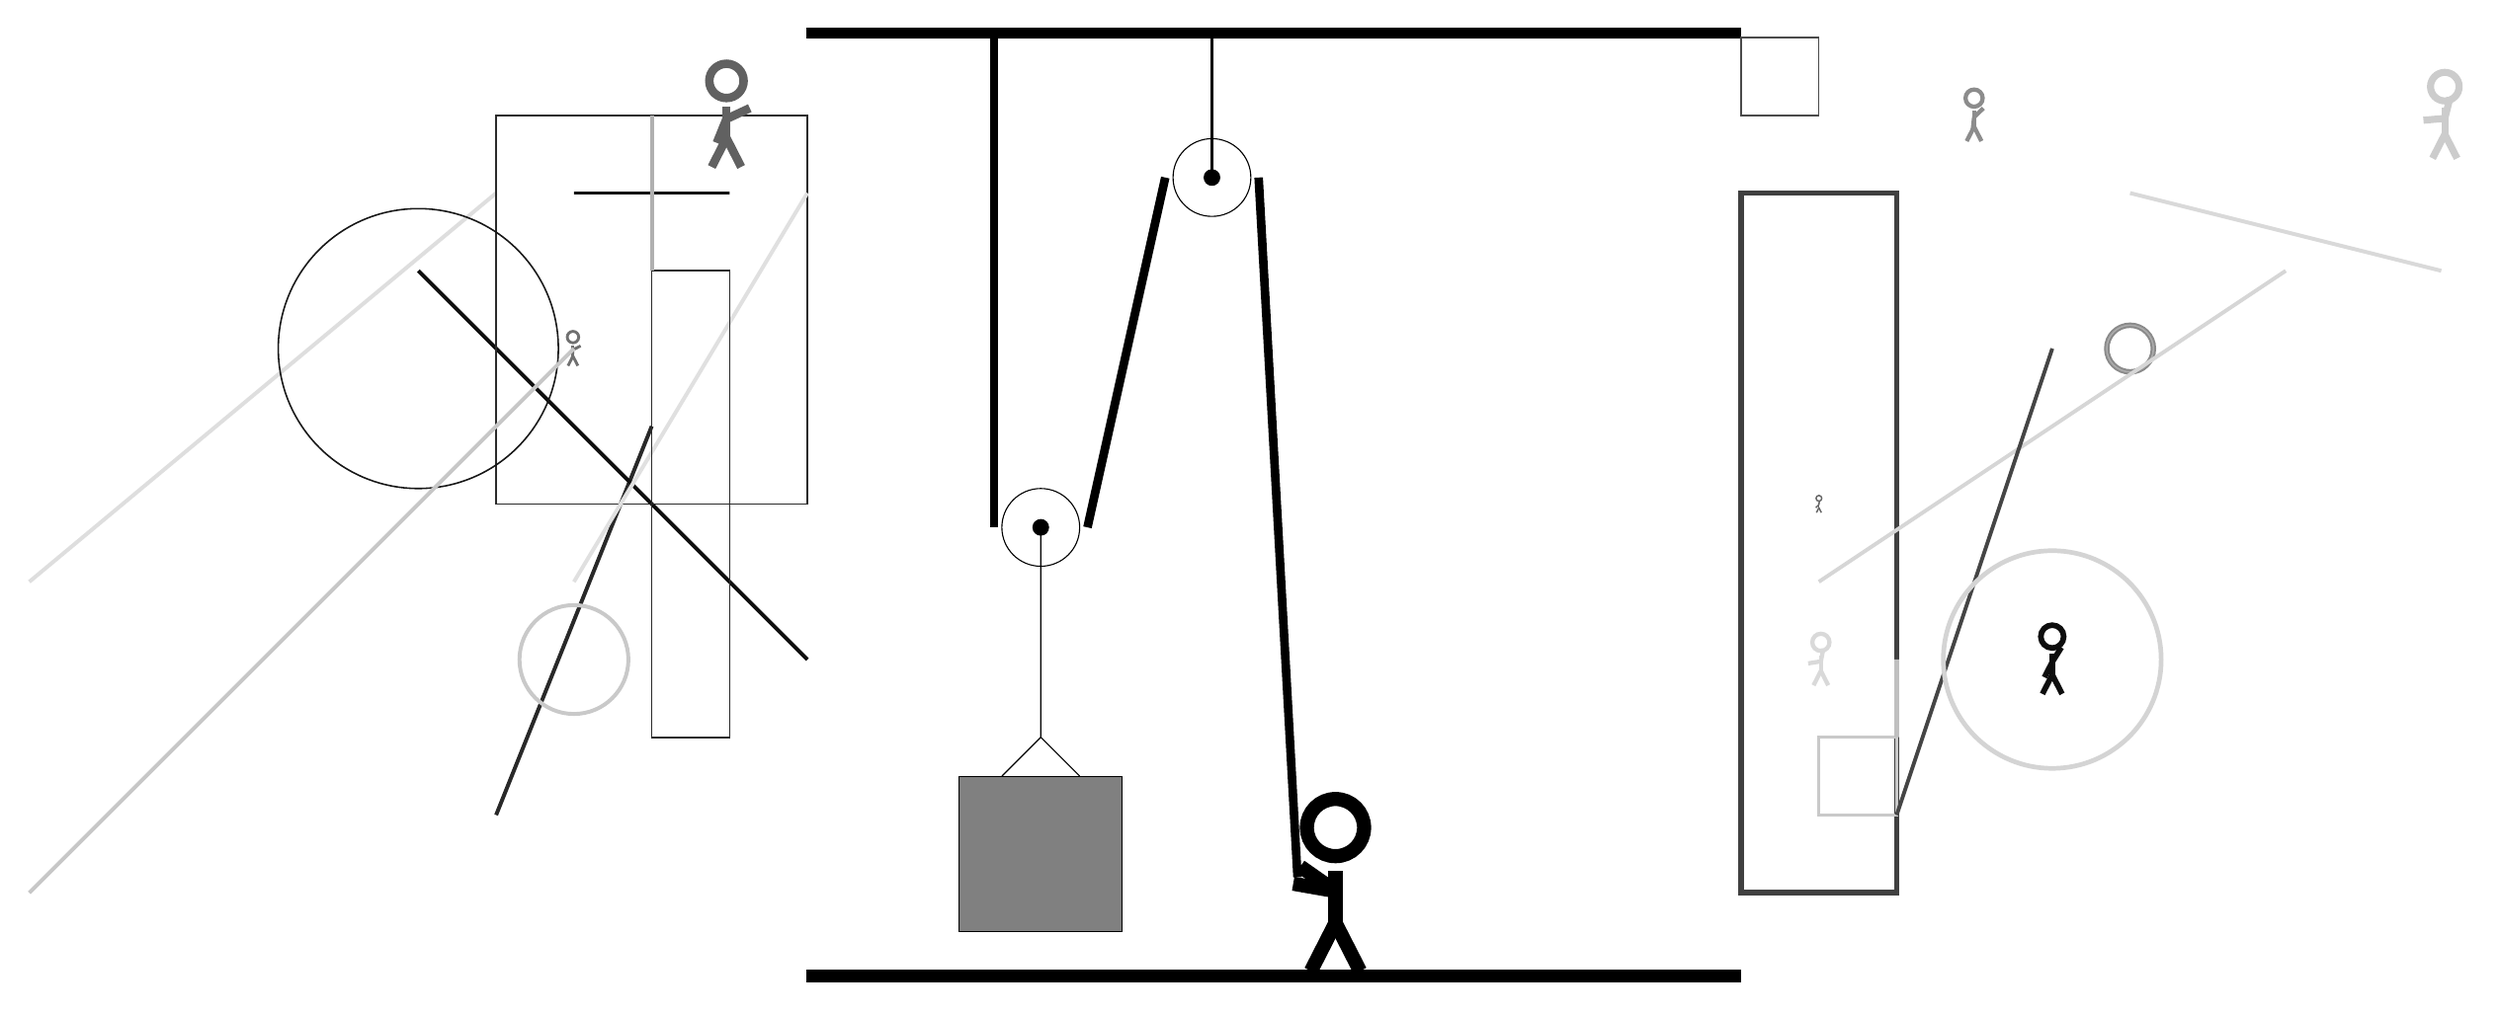
\begin{tikzpicture}
			%%%%% START %%%%%
			
			\draw[fill=black] (-2, 9) rectangle (10, 9.125);
			
			\draw (3.2, 7.2) circle (0.5);
			\draw[fill=black] (3.2, 7.2) circle (0.1);
			\draw[thick] (3.2, 7.2) -- (3.2, 9);
			
			\draw (1, 2.7) circle (0.5);
			\draw[fill=black] (1, 2.7) circle (0.1);
			
			\draw[line width=0.7mm, color=black!75] (12, -2) rectangle (10, 7);
			
			\draw[line width=0.5mm, color=black!84](-4, 4) -- (-6, -1);
			\draw[line width=0.2mm, color=black!71] (10, 9) rectangle (11, 8);
			\draw [line width=0.7mm, color=black!46](15, 5) circle (0.3);
			\node[line width=0.4mm, color=black!45] at (13, 8) {\Strichmaxerl[3][84][44]};
			\draw[line width=0.5mm, color=black!13](-6, 7) -- (-12, 2);
			\draw [line width=0.2mm, color=black!33](15, 5) circle (0.3);
			\node[line width=0.2mm, color=black!15] at (11, 1) {\Strichmaxerl[3][9][79]};
			\draw[line width=0.5mm, color=black!94](-7, 6) -- (-2, 1);
			\node[line width=0.4mm, color=black!56] at (-5, 5) {\Strichmaxerl[2][86][27]};
			
			\draw[line width=0.5mm, color=black!15](15, 7) -- (19, 6);
			
			\draw[line width=0.5mm, color=black!16](11, 2) -- (17, 6);
			\draw[line width=0.2mm, color=black!83] (-2, 3) rectangle (-6, 8);
			\draw[line width=0.5mm, color=black!12](-2, 7) -- (-5, 2);
			\draw[line width=0.4mm, color=black!21] (11, 0) rectangle (12, -1);
			\draw[line width=0.5mm, color=black!73](12, -1) -- (14, 5);
			
			\node[line width=0.7mm, color=black!60] at (11, 3) {\Strichmaxerl[1][45][82]};
			
			\draw [line width=0.6mm, color=black!17](14, 1) circle (1.4);
			\draw [line width=0.5mm, color=black!21](-5, 1) circle (0.7);
			\draw [line width=0.2mm, color=black!91](-7, 5) circle (1.8);
			\node[line width=0.6mm, color=black!62] at (-3, 8) {\Strichmaxerl[6][68][25]};
			
			\draw[line width=0.6mm, color=black!25] (12, 1) rectangle (12, 0);
			\node[line width=0.4mm, color=black!20] at (19, 8) {\Strichmaxerl[5][5][76]};
			\draw[line width=0.2mm, color=black!83] (-3, 0) rectangle (-4, 6);
			\draw[line width=0.5mm, color=black!22](-5, 5) -- (-12, -2);
			
			\node[line width=0.5mm, color=black!95] at (14, 1) {\Strichmaxerl[4][63][58]};
			\draw[line width=0.3mm, color=black!93] (-3, 7) rectangle (-5, 7);
			\draw[line width=0.5mm, color=black!31](-4, 6) -- (-4, 8);
			
			\draw (1, 2.7) -- (1, 0) -- (0.5, -0.5);
			\draw (1, 0) -- (1.5, -0.5);
			\draw[fill=black!50] (-0.05, -0.5) rectangle (2.05, -2.5);
			
			\draw[line width=1.1mm] (0.4, 9) -- (0.4, 2.7);
			\centerarc[line width=1.1mm](1, 2.7)(180:360:0.6);
			\draw[line width=1.1mm](1.6, 2.7) -- (2.6, 7.2);
			\centerarc[line width=1.1mm](3.2, 7.2)(0:180:0.6);
			\draw[line width=1.1mm](3.8, 7.2) -- (4.3, -1.8);
			
			\node at (4.7, -1.9) {\Strichmaxerl[10][-35][170]};
			
			\draw[fill=black] (-2, -3) rectangle (10, -3.15);
			
			%%%%% END %%%%%
		\end{tikzpicture}
	\end{figure}	
\end{document}